\documentclass[12pt]{extarticle}

\usepackage{graphicx}

\title{
	{\LARGE \bfseries Relating Electric Vehicle Ownership to Household Power Consumption}
}

\author{Scott Sullivan}

\begin{document}

\maketitle

\newpage

\section{Introduction}
What happens when someone plugs in their electric car?
The amount of power drawn from an electric vehicle (EV) can be higher than the peak usage of a typical househould.
Therefore, when someone plugs in their EV, the usage should noticeably spike.
By looking for spikes in household usage, it should be possible to infer properties of the data, such as which houses own EVs and when those EVs are charging.

By using techniques from statistics and machine learning, it was possible to predict which houses own EVs with an accuracy of $(84 \pm 2)\%$,
and when those houses were charging with an accuracy of $(93.0 \pm .6)\%$.
This paper describes at a high-level the techniques used to make these predictions.
Section II describes the Markov Model used to predict when an EV was charging.
Section III describes the K-Nearest-Neighbors (KNN) approach used to predict which houses own EVs.
Section IV describes other interesting features found in the data.
For more details, see the accompanying IPython Notebooks.

\section{When an EV is Charging}
In order to determine when an EV was charging, a Markov Model was constructed with hidden variables given by P(charging) and P(not charging), and observation variables given by the derivatives in the usage at each timestep.
The derivatives were found by using a cubic spline at each point in the data, and the first four derivatives were used as 4-Dimensional input (including the usage itself, the zeroth derivative).
Before the Markov Model was trained, each household's usage was normalized by subtracting its mean and dividing by its standard deviation.
Then the four sets of derivatives were normalized with each other by subtracting their overall mean and dividing by their deviation, in order to equalize the weights of each dimension.

The transition probabilities were calculated by separating each pair of adjacent timesteps into four groups: not charging $\rightarrow$ not charging (00), not charging $\rightarrow$ charging (01), charging $\rightarrow$ not charging (10), and charging $\rightarrow$ charging (11).
Then the derivatives at the second step in each transition were used to build a pair of 4D classifiers ($0 \rightarrow n$, $1 \rightarrow n$), which were used to predict $P(\mbox{charge}_i | \mbox{charge}_{i-1}, D_i)$, where $i$ was the timestep, and $D$ were the derivatives.
A plot showing the results of the Markov Model is shown in figure \ref{fig:markov}.
The overall accuracy of this method was $(93.0 \pm .06)\%$.
For more details, see Part II - Predicting When an EV is Charging.ipynb.

\begin{figure}
\centering
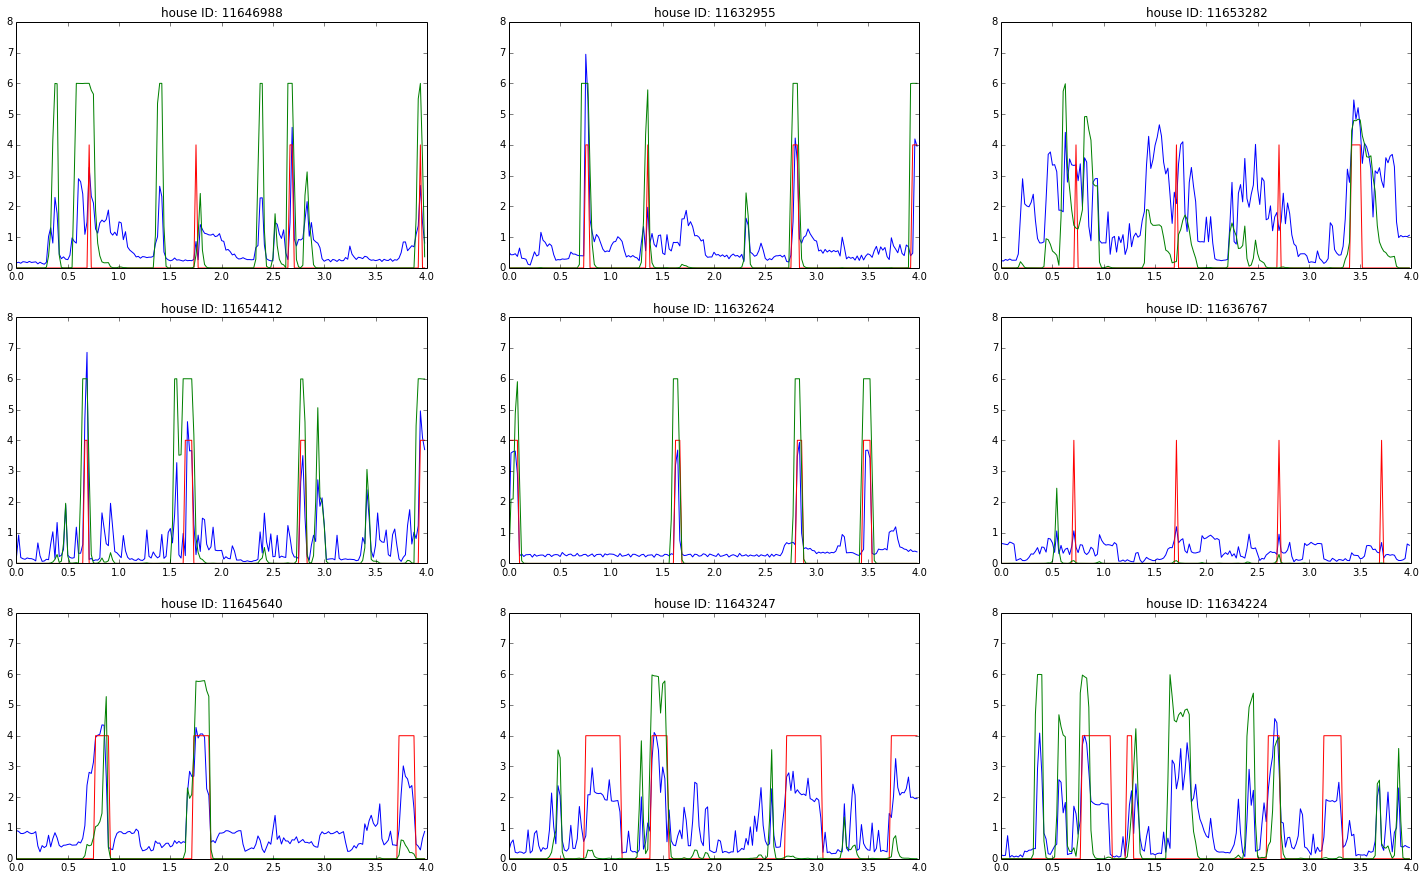
\includegraphics[width=15cm]{markov}
\caption{
Blue curve: Household usage (kWh/30-min interval), as a function of time (day).
Red curve: Times at which an EV is charging, scaled to 4 for visual clarity. 
Green curve: Probability an EV is charging as predicted by the Markov Model, scaled to 6 for visual clarity.
}
\label{fig:markov}
\end{figure}

\section{Which Houses Own EVs}
In order to determine which houses own EVs, a K-Nearest-Neighbor (KNN) classifier was constructed by calculating an array of statistical features for each household and experimentally testing which feature (or pair of features) contained the most predictive power.
The features included:
\begin{itemize}
	\item The average usage
	\item The standard deviation in the usage
	\item An average of the absolute values of the zeroth, first, second, and third derivatives
	\item Same as above, but increasing the influence of larger values by first taking the square, cube, 4th power, and 5th power of each point in the timeseries before averaging.
	\item Same as above, but after normalizing each usage graph first (as in section 2).
\end{itemize}
In addition, each feature was normalized with itself so they would all have the same weight.

A 1D KNN classifier was built for each feature, as well as a 2D KNN classifier for all possible pairs of features.
Because trying such a large number of different models was likely to result in overfitting, the data was split into train, validation, and test data.
The validation data was used to select the most accurate 1D KNN and the most accurate 2D KNN.
The test data was then used to gauge the true accuracy of each model by running once for the most accurate 1D KNN and once for the most accurate 2D KNN.

The most accurate classifier was the 1D KNN for average first derivative, weighted with k=5, with no household normalization.
The most accurate 1D KNN was actually more accurate than the most accurate 2D KNN.
It's likely all the pairs of features were not truly independent, causing models based on pairs of features to lose accuracy if the second statistic was not as powerful as the first.
A histogram of this feature is shown in figure \ref{fig:knn}.
The overall accuracy of this method was $(84 \pm 2)\%$.
For more details see Part III - Predicting Which Houses Own EVs.ipynb.

\begin{figure}
\centering
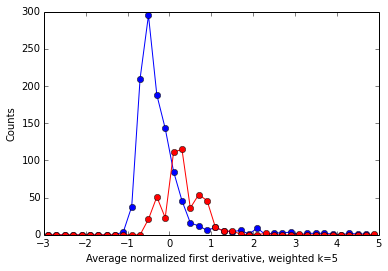
\includegraphics[width=8cm]{knn}
\caption{Histogram of \textbf{$\mbox{average}(|\mbox{usage first derivative}|^5)$}, separated into households without EVs (blue) and with EVs (red).}
\label{fig:knn}
\end{figure}

\section{Other Interesting Features in the Data}
During the analysis, several noteworthy features were found in the dataset which are described below.
The first was how much power an EV consumed on average.
To determine EV power consumption, first the base usage of each house was calculated by averaging all the usages when the EV was not charging.
This was then subtracted from each usage during charging, and the resulting usages were averaged for each house.
(The ends of each charge were also cut off, to remove times which were not charging for the complete interval).
It turns out the EV power consumption had two peaks, as seen in figure \ref{fig:power}.
It seems that there are two models of EV, one which consumes about 3.5 kW when plugged in, and one which consumes about 6.5 kW.

\begin{figure}
\centering
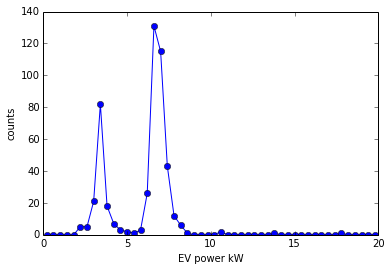
\includegraphics[width=8cm]{power}
\caption{Histogram of EV power consumption by household.}
\label{fig:power}
\end{figure}

The other intesting feature was the usage for each interval averaged across households.
A day/night cycle is clearly visible, as shown in figure \ref{fig:daynight}.
For more details, see Part IV - Other Intersting Features in the Data.ipynb.

\begin{figure}
\centering
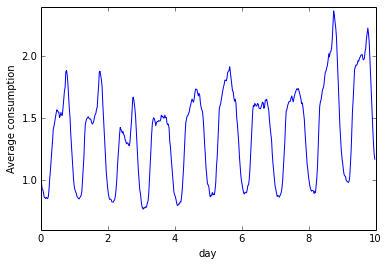
\includegraphics[width=8cm]{daynight}
\caption{Average household consumption over time.}
\label{fig:daynight}
\end{figure}


\section{Calculating Accuracies and Uncertainties}
The predictions in sections 2 and 3 were binary.
For example, the predictions in section 2 were whether a house was charging or not, which could be labeled as 0 for not charging and 1 for charging.
The predictions in section 3 were whether a house owned an EV, which could be labeled as 0 for no EV ownership and 1 for EV ownership.
If the classifier outputed 0 and the true result was 0, this would be labeled as a True Negative (or TN).
There exist definitions for all four possibilities, as described in the table below.
\\

\begin{center}
\begin{tabular}{ | l | l | l | l | }
	\hline
	Prediction & True Value & Name & Abbreviation \\ \hline
	0 & 0 & True Negative & TN \\ \hline
	0 & 1 & False Negative & FN \\ \hline
	1 & 0 & False Positive & FP \\ \hline
	1 & 1 & True Positive & TP \\
	\hline
\end{tabular}
\end{center}

The accuracy can be calculated using
\begin{equation}
\mbox{Accuracy} = (\mbox{TN} + \mbox{TP}) / (\mbox{TN} + \mbox{TP} + \mbox{FN} + \mbox{FP}).
\end{equation}
Other types of accuracies, such as the Positive Accuracy Rate and Negative Accuracy Rate, are calculated in Part II and Part III of the notebooks.

Since each of these four quantities is a count, the uncertainties were assumed to be Poissonian, which were calculated by taking the square root of each count.
The uncertainties were then propagated using partial derivatives.

The only exception was the accuracy of the Markov Model in section 2.
Since the accuracy of the Markov Model varied signficantly with each house, this variance was taken as the dominant uncertainty.
The overall accuracy was found by averaging each house's accuracy, while the uncertainty was taken as the standard deviation of the houses' accuracies and dividing by $\sqrt{N}$.

\end{document}
